
このチュートリアルでは、図 \ref{fig:tutrial_real_domain}に示した
領域を対象とした現実大気実験を行う。
現実大気実験用のチュートリアルは、下記で行う。
\begin{verbatim}
 scale/scale-rm/test/tutorial/real/
\end{verbatim}
これ以降の説明では、\verb|scale/scale-rm/test/tutorial/|の絶対PATHを
\verb|${Tutrial_DIR}|と示すこととする。
\verb|${Tutrial_DIR}|以下のディレクトリ構造は下記の通りである。
\begin{verbatim}
  init/
  net2g/
  pp/
  run/
  sample/  : サンプルのconfファイル
  tools/   : tutrial実行のためのツール
\end{verbatim}

SCALE-RMの実行過程は、図\ref{fig:howto}に示されるように
\begin{enumerate}
\item pp    : 地形・土地利用データの作成
\item init  : 初期値・境界値データの作成
\item run   : 時間積分を行う(モデル本体の実行)
\item net2g : 出力データのNetCDFからGrADS形式への変換(オプション) 
\end{enumerate}
といった手順で実行する。


\begin{figure}[h]
\begin{center}
  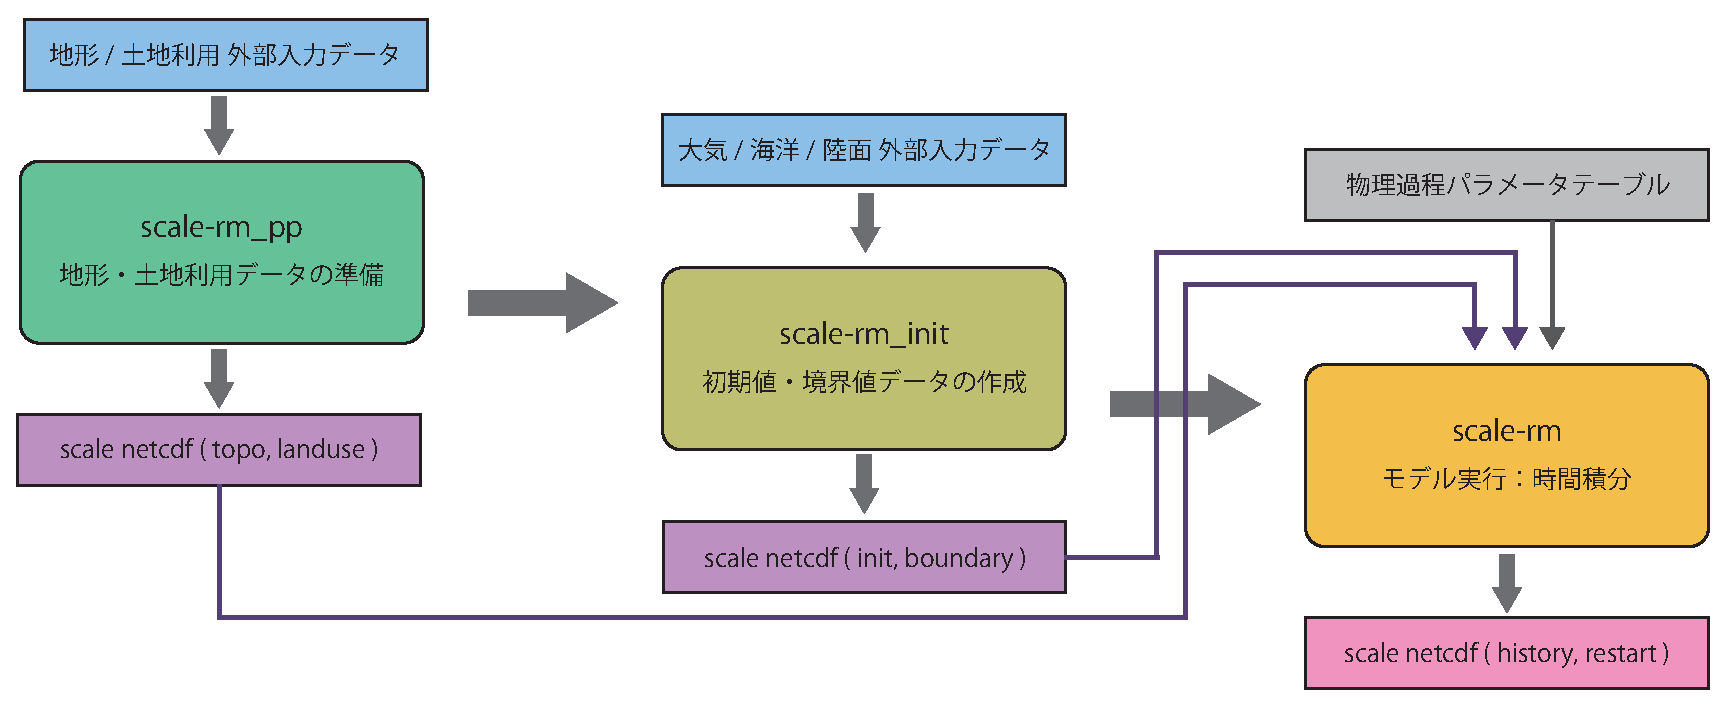
\includegraphics[width=0.9\hsize]{./figure/real_procedure.eps}\\
  \caption{SCALE-RMモデルの実行過程}
  \label{fig:howto}
\end{center}
\end{figure}

計算領域(ドメイン)の設定は表\ref{tab:grids}のようになっている。
チュートリアルは、SCALEの使い方を学ぶことが目的であり、
短い時間で実行可能な設定にしている。
領域モデルの実験設定として必ずしも適切な設定を選択しているとは限らないので
(例えば、15kmの水平解像度で積雲パラメタリゼーションなし)
ご留意頂きたい。

このチュートリアルを実行するには、下記の条件を満たす計算機環境が推奨される。
\begin{itemize}
\item CPU: 2コア/4スレッド以上の演算コアを持つCPU(4コア以上を推奨)
\item Memory容量: 4GB以上をプログラムに割当可能(8GB以上を搭載した計算機を推奨)
\item HDD空き容量: 7GB以上の空き容量
\end{itemize}
本節の説明で使用した環境は次のとおりである。
\begin{itemize}
\item CPU: Intel Xeon E5-2620 2.0GHz 6コア(ただし4コアのみ使用)
\item Memory: DDR3-1333 (4 channel, 32GB搭載)
\item OS: CentOS 6.6 x86-64, CentOS 7.1 x86-64, openSUSE 13.2 x86-64
\end{itemize}

\begin{figure}[tb]
\begin{center}
  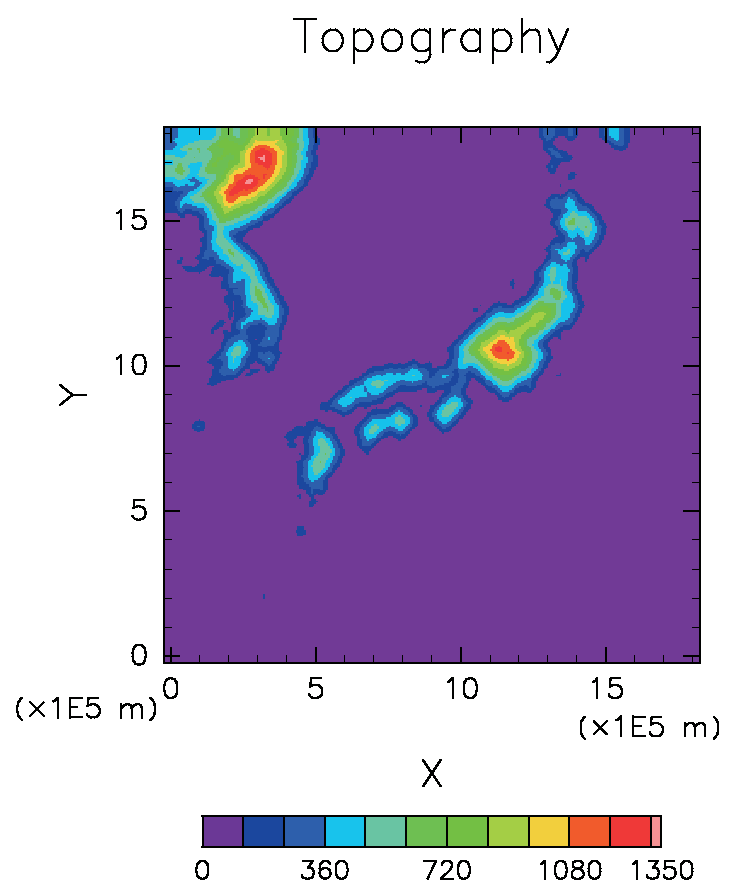
\includegraphics[width=0.5\hsize]{./figure/real_domain.eps}\\
  \caption{計算領域.カラーシェードは地形の標高を示す.}
  \label{fig:tutrial_real_domain}
\end{center}
\end{figure}

\begin{table}[h]
\begin{center}
  \caption{実験設定の概略}
  \label{tab:grids}
  \begin{tabularx}{150mm}{|l|X|} \hline
    \rowcolor[gray]{0.9} 項目 & 設定 \\ \hline
    MPIプロセス分割 (東西 x 南北) & 2 x 2 (合計4プロセス) \\ \hline
    水平格子数 (東西 x 南北) & 60格子点 x 60格子点 \\ \hline
    鉛直層数                 & 36層                  \\ \hline
    水平格子間隔             & dx = dy = 15km       \\ \hline
    積分期間 & 2014年8月10日 00UTC~12UTC (12時間積分) \\ \hline
    時間ステップ間隔 & 60 sec (720 steps) \\ \hline
  \end{tabularx}
\end{center}
\end{table}


%-------------------------------------------------------%
\section{境界データの準備}
%-------------------------------------------------------%

現実大気実験のシミュレーションを行う場合、SCALE本体に加えて
境界値データが必要になる。境界値データとしては表\ref{tab:real_bnd}
が必要である。{\color{blue}青字}は必須の変数、その他は任意である。

\begin{table}[h]
\begin{center}
  \caption{現実大気実験に必要な初期値境界値データ}
  \label{tab:real_bnd}
  \begin{tabularx}{150mm}{llX} \hline
    \multicolumn{3}{l}{地形データ(SCALE-RMの地形を用意する)}\\ \hline
    & \multicolumn{2}{l}{\color{blue}{標高データ}}\\
    & \multicolumn{2}{l}{\color{blue}{土地利用データ}}\\ \hline
    \multicolumn{3}{l}{初期値境界値データ}\\ \hline
    &  \multicolumn{2}{l}{\color{blue}{親モデルの緯度・経度}}\\
    &  \multicolumn{2}{l}{(3次元大気データ)}\\
    & &  \multicolumn{1}{l}{\color{blue}{東西風速, 南北風速, 気温, 比湿(相対湿度), 気圧, ジオポテンシャル高度}} \\
    &  \multicolumn{2}{l}{(2次元大気データ)}\\
    & & 海面更正気圧, 地上気圧, 10m東西風速, 10m南北風速, 2m気温, 2m比湿(相対湿度) \\
    &  \multicolumn{2}{l}{(2次元陸面データ)}\\
    & &  \multicolumn{1}{l}{親モデルの海陸マップ}\\
    & &  \multicolumn{1}{l}{\color{blue}{地表面温度}}\\
    & &  \multicolumn{1}{l}{{\color{blue}{親モデル土壌データの深さ情報, 土壌温度}}, 土壌水分(体積含水率 or 飽和度)}\\
    &  \multicolumn{2}{l}{(2次元海面データ)}\\
  & &  \multicolumn{1}{l}{海面水温}\\ \hline
  \end{tabularx}
\end{center}
\end{table}


\subsubsection{地形データと土地利用データ}
標高データと土地利用データは実験設定に従って、
SCALEのそれぞれの格子点における地形、海陸分布、土地利用を
作成するために使用する。
ユーザーが全球の任意の地域を対象とした計算ができるよう、
フォーマット変換済みの
標高データ USGS(U.S. Geological Survey) のGTOPO30 と、
土地利用データ GLCCv2 を提供している。

\begin{enumerate}
\item データのダウンロード\\
SCALE用の地形・土地利用のデータを\\
 \url{http://scale.aics.riken.jp/download/scale_database.tar.gz}\\
より入手し、任意のディレクトリに展開しておく。
\begin{verbatim}
  $ tar -zxvf scale_database.tar.gz
\end{verbatim}
展開したディレクトリには、地形データと土地利用データが格納されている。
\begin{verbatim}
  scale_database/topo/    <- 地形データ
  scale_database/landuse/ <- 土地利用データ
\end{verbatim}

\item パスの設定\\
makeを使ったジョブスクリプトを使用する場合には、
展開先のディレクトリを \verb|SCALE_DB| という環境変数に設定しておくと便利である
(以後、\verb|${SCALE_DB}|と表記)。
\begin{verbatim}
  $ export SCALE_DB=${path_to_directory_of_scale_database}/scale_database
\end{verbatim}
\end{enumerate}

\subsubsection{大気・陸面・海面水温データ}
\label{sec:real_prep}
初期値境界値データは4-byte バイナリー(grads format)に変換すれば、
任意のデータを読み込むことが可能である。
チュートリアルではNCEP FNL(Final) Operational Global Analysis dataを使用する。
\begin{enumerate}
\item データのダウンロード\\
NCARのサイト
 \url{http://rda.ucar.edu/datasets/ds083.2/}\\
から、2014年8月10日のgrib2フォーマットのデータ
\begin{verbatim}
  fnl_20140810_00_00.grib2
  fnl_20140810_06_00.grib2
  fnl_20140810_12_00.grib2
  fnl_20140810_18_00.grib2
\end{verbatim}
を\verb|${Tutrial_DIR}/real/tools/|の下にダウンロードする。

\item データフォーマットをgribからbinaryに変換\\
 SCALEは4byte バイナリー(grads format)の境界値データを読み込むことができる。\\
\verb|${Tutrial_DIR}/real/tools/| の中にある \verb|convert_grib2grads.sh|を実行。
ただし、あらかじめ\verb|wgrib2|がインストールされている必要がある.
\begin{verbatim}
  $ sh convert_grib2grads.sh
\end{verbatim}
成功すれば、下記のファイルが作成される。
\begin{verbatim}
  $ ls FNL_output/*/*
     FNL_output/201408/FNLatm_2014081000.grd
     FNL_output/201408/FNLatm_2014081006.grd
     FNL_output/201408/FNLatm_2014081012.grd
     FNL_output/201408/FNLatm_2014081018.grd
     FNL_output/201408/FNLland_2014081000.grd
     FNL_output/201408/FNLland_2014081006.grd
     FNL_output/201408/FNLland_2014081012.grd
     FNL_output/201408/FNLland_2014081018.grd
     FNL_output/201408/FNLsfc_2014081000.grd
     FNL_output/201408/FNLsfc_2014081006.grd
     FNL_output/201408/FNLsfc_2014081012.grd
     FNL_output/201408/FNLsfc_2014081018.grd
\end{verbatim}
\end{enumerate}

